\chapter{经典场传播与数值可信度}
\label{ch:propagation}

\begin{learningobjectives}
完成本章后，读者应能：
\begin{enumerate}
  \item 为 TWA 场方程选择与边界条件相符的传播算法；
  \item 推导 Fourier 分步法并说明其二阶精度与可逆性；
  \item 用守恒量、步长标度、反向传播和独立实现检验数值可信度；
  \item 组织可复现的随机轨迹并区分积分误差、截止误差和抽样误差。
\end{enumerate}
\end{learningobjectives}

\section{轨迹方程与量子近似是两层问题}

TWA 把量子演化近似成确定性经典场轨迹的系综。以第10章的一维格点方程为例，写成
\begin{equation}
  \ii\hbar\partial_t\psi
  =\left[T+V(x,t)+g(t)(|\psi|^2-\delta_{\mathcal C}(x,x))\right]\psi,
  \qquad
  T=-\frac{\hbar^2}{2m}\partial_x^2.
  \label{eq:propagation-field-equation}
\end{equation}
有限步长算法求解的是这条轨迹方程；丢弃高阶 Moyal 项则是把量子问题变成该方程的近似。前者收敛并不证明后者正确，但前者不收敛时，任何量子解释都失去基础。
投影经典场计算中的数值实践、截止依赖与热化风险可进一步参见
\cite{Blakie2008}。

以下讨论以闭合系统的确定性 TWA 为主。若主方程在 Wigner 表示中产生扩散，轨迹会变为随机微分方程，必须另行指定 It\^o 或 Stratonovich 解释；不能把本章的常微分方程积分器直接套用。

下文为简化排版记
$\delta_{\mathcal C}(x)\equiv\delta_{\mathcal C}(x,x)$。只有在等距、完整的
Fourier--DVR 网格上它才是常数 $1/\Delta x$；陷阱本征态截断、非均匀网格
或其他投影基一般给出随位置变化的对角投影核。代码若把它硬编码成一个
标量，就等于额外假设了均匀模式密度。

\section{Strang 分裂 Fourier 法}

周期边界下，把右端拆成动能 $T$ 与局域项
\begin{equation}
  U[\psi;t]=V(x,t)+g(t)(|\psi|^2-\delta_{\mathcal C}(x)).
\end{equation}
对时间无关参数，一个步长 $\Delta t$ 的 Strang 分裂为
\begin{equation}
  \psi(t+\Delta t)
  \approx
  \ee^{-\ii T\Delta t/(2\hbar)}
  \ee^{-\ii U\Delta t/\hbar}
  \ee^{-\ii T\Delta t/(2\hbar)}\psi(t).
  \label{eq:strang-splitting}
\end{equation}
动能指数在 Fourier 空间对角：
\begin{equation}
  \tilde\psi_k\longleftarrow
  \exp\!\left[-\ii\frac{\hbar k^2}{2m}\frac{\Delta t}{2}\right]
  \tilde\psi_k.
  \label{eq:kinetic-half-step}
\end{equation}
局域子步中 $|\psi(x)|^2$ 不变，因此可以精确写成相位乘法
\begin{equation}
  \psi(x)\longleftarrow
  \exp\!\left[-\frac{\ii\Delta t}{\hbar}
  \left(V(x)+g(|\psi(x)|^2-\delta_{\mathcal C}(x))\right)\right]\psi(x).
  \label{eq:local-nonlinear-step}
\end{equation}

若 $V$ 或 $g$ 随时间变化，应在子步中使用中点值 $t+\Delta t/2$，以保持整体二阶精度。式\eqref{eq:strang-splitting}的局域截断误差是 $\order(\Delta t^3)$，固定总时长的全局误差是 $\order(\Delta t^2)$；时间分裂谱方法在 Gross--Pitaevskii 方程中的系统分析和网格选择可参见\cite{Bao2003}。对时间无关、无滤波的实现，三个子步都是幺正的，因而离散范数在浮点误差内守恒；将 $\Delta t$ 换成 $-\Delta t$ 并逆序执行还能恢复初态。

\begin{warningbox}
范数守恒是必要测试，却不是精度证明。分步法的每个子步都可以严格守范数，即使步长大到相位和能量已经完全错误。必须再做步长标度和能量检查。
\end{warningbox}

\section{其他积分器何时更合适}

\subsection{有限差分与 Runge--Kutta}

复杂边界、非局域耦合或无法对角化的单粒子哈密顿量可先离散成
$\dot{\bm y}=\bm f(t,\bm y)$，再用 Runge--Kutta 法。显式 RK4 易实现，但对高波数动能是刚性的：稳定步长常随 $\Delta x^2$ 缩小。自适应高阶法可以控制局域误差，却通常不严格保持 Hamilton 结构和守恒量。

\subsection{隐式与结构保持方法}

Crank--Nicolson 对线性 Schr\"odinger 方程范数稳定；非线性问题需迭代求解。辛积分器或离散梯度方法更适合极长时间守恒研究，但每步成本可能更高。选择算法应由 Hamilton 结构、边界条件和目标时间尺度决定，而不是只比较单步速度。

\subsection{耦合分量}

双分量场的动能常仍可在 Fourier 空间传播，局域子步则包含一个 $2\times2$ 自旋哈密顿量。若 Rabi 耦合与非线性密度项不对易，可以在局域子步中对矩阵指数做解析或数值计算，或继续采用对称分裂。第14章将给出具体模型。

\section{投影、混叠与边界}

实空间乘积 $|\psi|^2\psi$ 会产生输入最高波数三倍的 Fourier 分量。有限网格无法表示这些分量，它们会以混叠形式折回低波数。处理方式包括：
\begin{enumerate}
  \item 把伪谱格点方程本身视为所定义的有限维模型，并通过加密网格检查；
  \item 对乘积使用零填充和去混叠规则；
  \item 每次计算非线性后显式施加 $\mathcal P_{\mathcal C}$。
\end{enumerate}
显式滤波若不是方程的一部分，会损失范数和能量；必须把它当作模型操作记录，而不是隐藏在“数值稳定化”中。

周期 Fourier 法还会让离开右边界的波包从左边界返回。研究膨胀或散射时，应增大计算域、在目标时间前停止，或加入经过反射测试的吸收层。吸收势使系统非 Hermitian，粒子数下降是建模结果而非积分误差。

\section{守恒量与可逆性测试}

对时间无关的闭合单分量模型，至少监测
\begin{align}
  \mathcal N_{\mathrm{sym}}&=\int\dd x\,|\psi|^2,\\
  N_W&=(\hat N)_W=\mathcal N_{\mathrm{sym}}-\frac M2,\\
  E_W&=\int\dd x\left[
  \frac{\hbar^2}{2m}|\partial_x\psi|^2+V|\psi|^2
  +\frac{g}{2}\left(|\psi|^4-2\delta_{\mathcal C}(x)|\psi|^2\right)
  \right],
  \label{eq:propagation-weyl-energy}
\end{align}
其中省略了不影响动力学的常数。$\mathcal N_{\mathrm{sym}}$ 是单条 Wigner
轨迹的原始对称范数；$N_W$ 才是扣除每模半量子后的粒子数 Weyl 符号，且
$\qavg{\hat N}=\ensavg{N_W}$。两者漂移相同，但输出时不能混用名称。

建议记录最大相对漂移而不只记录末时误差：
\begin{equation}
  \epsilon_Q=\max_{0\le t\le t_f}
  \frac{|Q(t)-Q(0)|}{\max(|Q(0)|,Q_{\rm scale})}.
  \label{eq:conservation-error}
\end{equation}
$Q_{\rm scale}$ 防止近零守恒量令相对误差失真。再做反向传播：从 $t_f$ 用 $-\Delta t$ 返回，测量
\begin{equation}
  \epsilon_{\rm rev}=
  \frac{\|\psi_{\rm back}-\psi_0\|_2}{\|\psi_0\|_2}.
  \label{eq:reversibility-error}
\end{equation}
该测试对 FFT 归一化、子步顺序和隐式滤波尤其敏感，但仍不能替代与精细步长解的比较。

\section{步长与空间收敛}

对二阶算法，分别用 $\Delta t,\Delta t/2,\Delta t/4$ 得到同一时刻的场。若进入渐近区，误差比应接近
\begin{equation}
  \frac{\|\psi_{\Delta t}-\psi_{\Delta t/2}\|}
       {\|\psi_{\Delta t/2}-\psi_{\Delta t/4}\|}
  \simeq 2^2=4.
  \label{eq:second-order-ratio}
\end{equation}
非线性相位可能让整体相位误差主导，因此还应对密度、关联函数等目标观测量重复这一检查。

空间收敛必须固定清楚比较对象。加密格点会改变 TWA 模式数和初始半量子总量；若目的是测试离散算符，可先关闭随机噪声并传播同一光滑场。若目的是测试完整 TWA 预测，则应按各自截止重新抽样，并比较物理估计器的系综统计量。两种实验回答不同问题。

\section{轨迹系综与随机数管理}

轨迹天然可并行，但可复现并不等于所有进程使用同一个种子。重复种子会制造完全相同的轨迹并虚增名义样本数。可靠方案是从一个主种子派生互不重叠的子流，例如用计数型生成器或 \texttt{SeedSequence.spawn}。每条轨迹的标识、子流编号、参数哈希和代码版本都应写入元数据。

在比较两个参数或两种算法时，使用共同随机数可以显著降低“差值”的方差：两次计算采用同一组初态样本，但各自独立传播。这样得到的两个均值是相关的，误差条必须基于逐轨迹差值计算，不能套用独立样本公式。

自适应积分会让不同轨迹具有不同内部时间点。观测量应在统一输出网格上由积分器插值，避免把相邻但不相同的时间混入一个系综平均。

\section{实际分步传播基准}

配套程序用一条带固定随机种子的格点 Wigner 场验证 Strang 分裂。它同时测量范数漂移、Weyl 能量漂移、正反传播误差和四档步长的二阶收敛，结果见\cref{fig:split-step-benchmark}。
\begin{figure}[htbp]
  \centering
  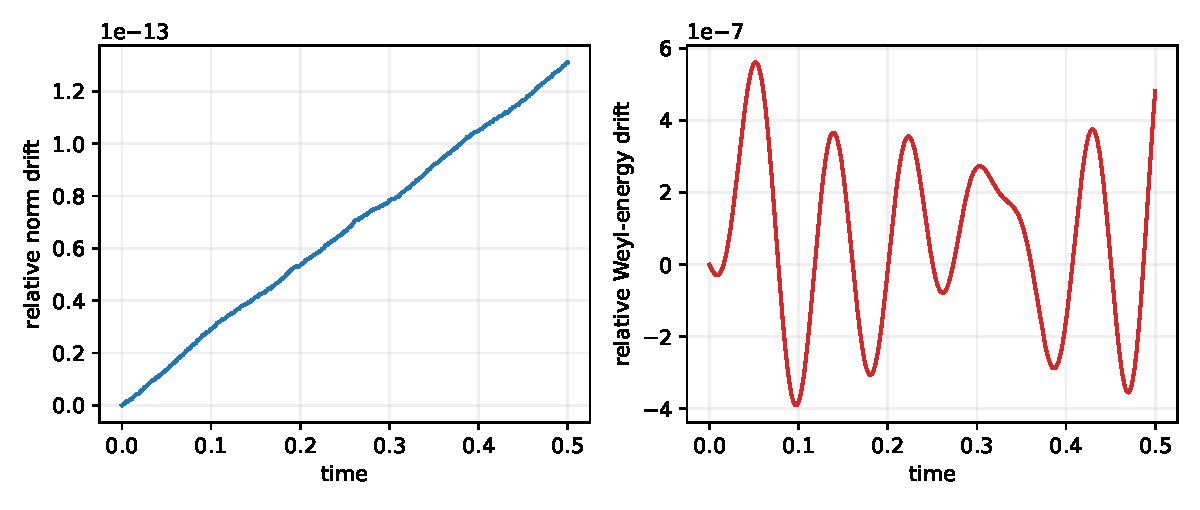
\includegraphics[width=0.78\textwidth]{figures/ch12/split_step_conservation.pdf}
  \caption[Strang 分裂传播的收敛与守恒基准]{周期区间 $L=20$ 上 $M=64$ 点单轨迹 Strang 分裂基准。步长 $\Delta t=0.004,0.002,0.001,0.0005$ 给出观测收敛阶 $2.001$；在记录步长 $\Delta t=0.001$ 下，范数漂移为 $1.31\times10^{-13}$、离散 Weyl 能量相对漂移为 $5.61\times10^{-7}$，正反传播误差为 $2.29\times10^{-13}$。该图验证离散积分器及其实现，不验证 TWA 的物理截断误差。}
  \label{fig:split-step-benchmark}
\end{figure}
这张图来自实际 FFT 传播；参数和误差保存在
\path{data/ch12/split_step_metrics.json}。该程序验证的是数值积分器，不是 TWA 对某个实验体系的物理准确性。

\begin{chaptercheck}
对每次生产运行保存四类互不替代的证据：时间步长表、空间/截止表、守恒与可逆性曲线、轨迹数与置信区间表。若只保存一条“结果曲线”和最终参数，事后无法判断偏差来自量子截断、数值积分还是 Monte Carlo 抽样。
\end{chaptercheck}

\section*{本章小结}

分步 Fourier 法利用动能和局域非线性的结构构造二阶、范数保持且可逆的传播，但仍需能量、步长标度和反向传播验证。投影、混叠、边界和随机数子流都是方程定义与可复现性的一部分。轨迹方程的数值收敛与 TWA 的量子有效性必须分别建立证据。

\begin{exercises}
  \item 用 Baker--Campbell--Hausdorff 公式说明对称分裂为何没有 $\order(\Delta t^2)$ 的单步误差项。
  \item 推导中心差分动能下显式 RK4 的稳定步长为何随 $\Delta x^2$ 缩小。
  \item 给式\eqref{eq:propagation-field-equation}加入时间依赖 $g(t)$，设计保持二阶精度的中点算法。
  \item 构造一个范数守恒但相位明显错误的大步长例子。
  \item 为双分量 Rabi 耦合的局域子步写出 $2\times2$ 矩阵指数。
\end{exercises}
